For your postlab \#2 assignment, use the REPL to create a 400 x 300 pixel window, just as you did in Part \#3 of your lab assignment, and then do your best to recreate the following graphics:

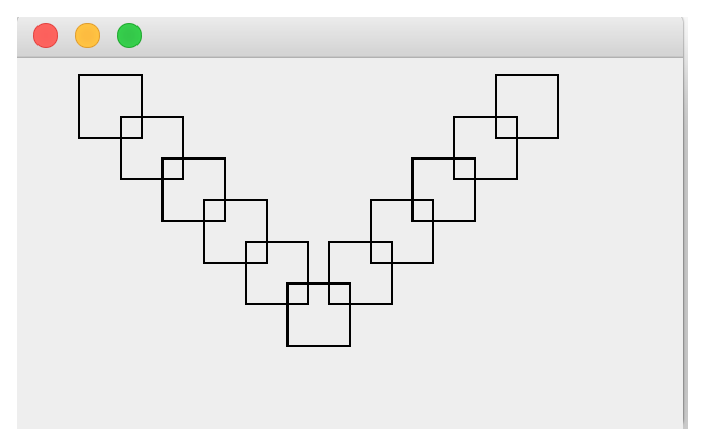
\includegraphics[scale=1]{lab2/lab2ss.eps} 

The clever way to solve this problem is to use variables to represent the locations / sizes of the rectangles. If you do this right, you should be able to mostly repeat the same statement or statements several times to draw the picture. You should do this ``the clever way'' for full credit, though simply getting a very similar result will be good enough for an A-. 

If you make mistakes and want to start over, use the /reset command in the REPL to return everything back to the original state. 

Once you're happy with the appearance of your artwork, enter the following command in to the REPL:

\begin{verbatim}
/save postlab2.txt
\end{verbatim}

Check to make sure this file contains all of your work from the REPL, then 
turn it in on the postlab \#2 assignment. 
